\documentclass{beamer}

\usepackage[slovene]{babel}
\usepackage[T1]{fontenc}
\usepackage[utf8]{inputenc}
\usepackage{lmodern}

\usepackage{amssymb}
\usepackage{amsmath}

\usepackage{enumerate}
\usepackage{graphicx}

\usetheme{Ilmenau}
\usecolortheme{beaver}

\setbeamercolor{block title}{bg=darkred,fg=structure.fg!20!bg!50!bg}
%\setbeamercolor{block body}{bg=white}

\DeclareMathOperator {\stopnja} {deg}

\title{Problem londonskega stolpa}
\author[Ines Meršak]{Ines Meršak \\[5px] mentor: prof. dr. Sandi Klavžar}
\date{16.~11.~2015}

\begin{document}
    
\begin{frame}[plain]
    \titlepage
\end{frame}

%\begin{frame}
%    Kratka predstavitev:
%    \begin{itemize}
%        \item klasičen problem londonskega stolpa - opis igre
%        \item osnovne definicije teorije grafov
%        \item klasičen problem londonskega stolpa - lastnosti grafa (Hamiltonova pot, etc.)
%        \item posplošen londonski stolp - definicija, povezanost, planarnost
%        \item primeri uporabe v psihologiji
%    \end{itemize}
%\end{frame}

\section{Klasični problem londonskega stolpa}
\begin{frame}{Klasični problem londonskega stolpa (Shallice)}
    \begin{figure}
        \centering
        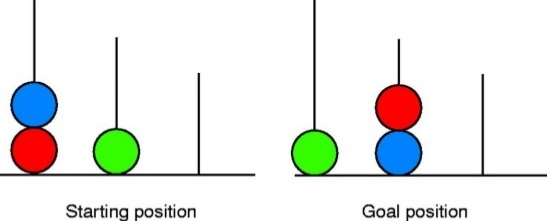
\includegraphics[height=70pt]{img/tol.jpg}
    \end{figure}
    \begin{itemize}
        \item izumljen leta 1982
        \item 3 enako velike krogle različnih barv
        \item 3 palice različnih velikosti
        \item cilj igre je priti iz trenutnega stanja v neko dano stanje z minimalnim številom potez
        \item najboljši način za vizualizacijo tega problema je s pomočjo grafov
    \end{itemize}
\end{frame}

\begin{frame}{Osnovne definicije teorije grafov}
    \begin{itemize}
        \item graf $ G = (V, E) $
        \item \alert{soseščina} vozlišča $u$ je $N(u) = \{x \in V;\ ux \in E\}$
        \item \alert{stopnja} vozlišča $u$: $\stopnja u  = \lvert N(u) \rvert$
        \item \alert{sprehod} v grafu je zaporedje vozlišč $v_1,\ldots v_k$, da za vsak $i$ velja $v_i v_{i+1} \in E$
        \item graf je \alert{povezan}, če za poljuben par vozlišč obstaja sprehod med njima
        \item \alert{diameter} grafa je najmanjše maksimalno število povezav, ki jih moramo prepotovati, da pridemo od poljubnega vozlišča do nekega drugega vozlišča v temu grafu
    \end{itemize}
\end{frame}

\begin{frame}
    \begin{itemize}
        \item \alert{ravninski} graf je graf, ki ga lahko narišemo v ravnini brez križanja povezav
        \item pot v grafu, ki vsebuje vsa vozlišča, je \alert{Hamiltonova pot}
    \end{itemize}
\end{frame}

\begin{frame}{Graf klasičnega problema londonskega stolpa}
%    Označimo krogle s številkami 1, 2, 3, pri čemer je npr.\ krogla 1 modra, krogla 2 rdeča, krogla 3 pa rumena. Začetek nove palice bomo nakazali z |, krogle pa bomo naštevali od vrha proti dnu palice.
    
    \begin{figure}
        \centering
        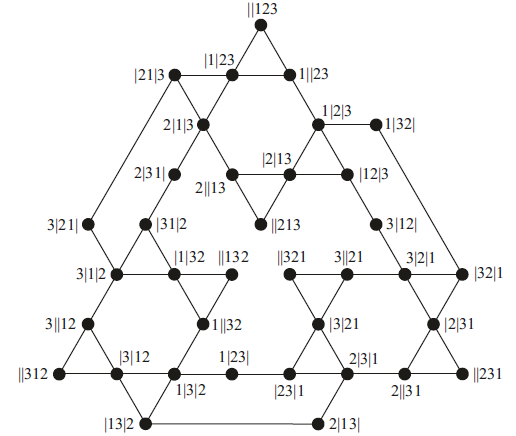
\includegraphics[height=190pt]{img/tolgraph.png}
    \end{figure}
\end{frame}

\begin{frame}{Lastnosti grafa}
    \begin{itemize}
        \item 36 vozlišč (36 možnih stanj)
        \item utežene stopnje vozlišč
        \item diameter grafa je 8
        \item ravninski
        \item vsebuje Hamiltonovo pot
    \end{itemize}
\end{frame}

\section{Posplošen londonski stolp}
\begin{frame}{Oznake}
%    \begin{itemize}
%        \item J.\ R.\ Tunstall prvi predlagal razširitev na 4 krogle s podaljšanimi palicami
%    \end{itemize}
    Imamo $p$ palic in $n$ krogel različne barve, pri čemer je $p \geq 3 \text{ in } n \geq 2$. Vsako palico označimo s številom $k \in [p]$, pri čemer je $h_k$ višina palice. Veljati mora $n \leq \sum_{k=1}^p h_k$. Poteza je veljavna, če vrhnjo kroglo neke palice prestavimo na vrh druge, pod pogojem, da je na tej palici manj kot $h_k$ krogel.
    
    Vsako stanje krogel lahko enolično predstavimo s permutacijo $s \in S_{n+p}$.
\end{frame}

\begin{frame}{Definicija}
    \begin{block}{Definicija}
        $p \geq 3,\ n \geq 2,\ h \in [n]^p,\  \sum_{k=1}^p h_k \geq n$. \\
        Množica vozlišč \alert{Londonskega grafa}, označimo ga z $L_h^n$, je sestavljena iz vseh $s \in S_{n+p}$, za katere velja:
        \[\forall k \in [p]:\ 1 \leq s_{n+k} - s_{n+k-1} \leq h_k + 1,\ s_{n+p} = n + p .\]
        Vsaka povezava Londonskega grafa je sestavljena iz takega para vozlišč, da lahko s pomočjo ene veljavne poteze pridemo iz stanja, ki pripada prvemu vozlišču, v stanje, ki pripada drugemu vozlišču.
    \end{block}

\end{frame}

\begin{frame}{Lastnosti grafa}
    Potreben pogoj za povezanost Londonskega grafa je 
    \[ n \leq \sum_{k=1}^{p-1} h_k. \]
    \begin{block}{Izrek}
        Londonski graf $L_h^n$ je povezan natanko tedaj, ko velja pogoj
        \[ n \leq \sum_{k=1}^{p-1} h_k. \]
    \end{block}
\end{frame}

\section{Uporaba}
\begin{frame}{Primeri uporabe}
    \begin{itemize}
        \item problem londonskega stolpa je bil razvit z namenom merjenja sposobnosti načrtovanja in reševanja problemov v bolnikih s poškodbami čelnega režnja možganov
        \item slabo reševanje londonskega stolpa se interpretira kot nezmožnost učinkovitega načrtovanja
        \item uporabljen za ocenjevanje napredka bolezni pri bolnikih z Alzheimerjevo in Parkinsonovo boleznijo
        \item uporabljen za opazovanje vedenja majhnih otrok pri reševanju problemov
    \end{itemize}
\end{frame}

\end{document}
